\documentclass[12pt]{article}
\usepackage{preamble}
\usepackage{longtable}

\geometry{a4paper, left=2.5cm, right=2.5cm, top=2cm, bottom=2.5cm}

\pagestyle{plain}

\newcommand{\placeholder}[1]{{\color{magenta}#1}}

\chead{
    \begin{minipage}{1\linewidth}
        \begin{wrapfigure}{r}{0pt}
            
\includegraphics[height=1cm]{images/logo}
        \end{wrapfigure}
        {
            \centering
            \sffamily\scriptsize
            \textbf{
                Санкт-Петербургский национальный исследовательский университет \\
                информационных технологий, механики и оптики}
            %th3p4g
            \vspace{2mm}

            \quad\quad\quad\quad\quad\quad\ \textbf{УЧЕБНЫЙ ЦЕНТР ОБЩЕЙ ФИЗИКИ ФТФ}
        }
    \end{minipage}
}



\begin{document}
    \vspace*{2\baselineskip}

    \thispagestyle{fancy}

    \noindent
    \textbf{Группа} \underline{\hspace{4.85cm}} \hfill \textbf{К работе допущен} \underline{\hspace{4cm}} \\[0.5cm]
    \textbf{Студент} \underline{\hspace{4.6cm}} \hfill \textbf{Работа выполнена} \underline{\hspace{4cm}} \\[0.5cm]
    \textbf{Преподаватель} \underline{\hspace{3.2cm}} \hfill \textbf{Отчет принят} \underline{\hspace{4.85cm}} \\


    \begin{center}
    {\huge \textbf{Рабочий протокол и отчёт по\\ лабораторной работе № \placeholder{X.YZ}}}

        \smallvspace

        {\Large \placeholder{Название лабораторной работы}}
    \end{center}


    \noindent
    1. \textbf{Цель работы.}

    \begin{enumerate}
        \item \placeholder{Цель №1}

        \item \placeholder{Цель №N}
    \end{enumerate}

    \mediumvspace

    \noindent
    2. \textbf{Задачи, решаемые при выполнении работы.}

    \begin{enumerate}
        \item \placeholder{Задача №1}

        \item \placeholder{Задача №2}

        \item \placeholder{Задача №N}
    \end{enumerate}

    \mediumvspace

    \noindent
    3. \textbf{Объект исследования.}

    \placeholder{Объект исследования}

    \mediumvspace

    \noindent
    4. \textbf{Метод экспериментального исследования.}

    \placeholder{Метод исследования}

    \mediumvspace

    \noindent
    5. \textbf{Рабочие формулы и исходные данные.}

    \begin{center}
    \textbf{Исходные данные}
\end{center}

\begin{flushleft}
    $\text{Масса каретки} \hspace{4.95cm} (47,0 \pm 0,5)\text{г}$ \\
    $\text{Масса шайбы} \hspace{5.2cm} (220,0 \pm 0,5)\text{г}$ \\
    $\text{Масса грузов на крестовине} \hspace{2.45cm} (408,0 \pm 0,5)\text{г}$ \\
    $\text{Расстояние первой риски от оси} \hspace{1.7cm} (57,0 \pm 0,5)\text{мм}$ \\
    $\text{Расстояние между рисками} \hspace{2.55cm} (25,0 \pm 0,2)\text{мм}$ \\
    $\text{Диаметр ступицы} \hspace{4.35cm} (46,0 \pm 0,5)\text{мм}$ \\
    $\text{Диаметр груза на крестовине} \hspace{2.15cm} (40,0 \pm 0,5)\text{мм}$ \\
    $\text{Высота груза на крестовине} \hspace{2.4cm} (40,0 \pm 0,5)\text{мм}$ \\
\end{flushleft}

\begin{center}
    \textbf{Рабочие формулы}
\end{center}

\text{Ускорение груза}
\[
a = \frac{2h}{t^2}
\]
Где:
\[
\text{$h$ - расстояние, пройденное грузом за время $t$ от начала движения}
\]

\text{Связь между угловым ускорением и линейным ускорением груза} 
\[
\varepsilon = \frac{2a}{d} = \frac{4h}{t^2d}
\]
Где:
\[
\text{$d$ — диаметр ступицы}
\]

\text{Момент силы натяжения нити}
\[
M = \frac{m d}{2} \left(g - a \right) = \frac{m d}{2} \left(g - \frac{2 h}{t^2} \right)
\]

\text{Основной закон динамики вращения}
\[
I \varepsilon = M - M_{\text{тр}}
\]
Где:
\begin{center}
    \text{$I$ — момент инерции крестовины} \\
    \text{$\varepsilon$ — угловое ускорение крестовины} \\
    \text{$M$ и $M_{\text{тр}}$ — моменты сил натяжения нити и трения на крестовине} \\
\end{center}

\begin{center}
    \text{В соответствии с теоремой Штейнера момент инерции крестовины зависит от расстояния} 
    \text{между центрами грузов и осью вращения по формуле}
\end{center} 
\[
I = I_0 + 4 m_{\text{ут}} R^2
\]
Где:
\begin{center}
    \text{$I_0$ - сумма моментов инерции стрежней крестовины, момента инерции ступицы} 
    \text{и собственных центральных моментов инерции утяжелителей}
\end{center}

\text{Момент инерции крестовины с утяжелителями по МНК} 
\[
I = \frac{\sum_{i=1}^{N} \left( \varepsilon_i - \overline{\varepsilon} \right) \left( M_i - \overline{M} \right)}{\sum_{i=1}^{N} \left( \varepsilon_i - \overline{\varepsilon} \right)^2}
\]

\text{Расстояние от оси крестовины до грузов-утяжелителей}: 
\[
R = l_1 + \left( n - 1 \right) l_0 + \frac{b}{2}
\]

Где:
\begin{center}
    \text{$l_1$ – расстояние от оси вращения до первой риски} \\
    \text{$n$ – номер риски, на которой установлены утяжелители} \\
    \text{$l_0$ – расстояние между соседним рисками} \\
    \text{$b$ – размер утяжелителя вдоль спицы} \\
\end{center}

\text{Момент инерции крестовины по т. Штейнера}
\[
I_0 = \overline{I} - 4m_{\text{ут}}\overline{R}^2
\]
Где:
\[
m_\text{ут} = \frac{\sum_{i=1}^{N} \left( R_i - \overline{R} \right) \left( I_i - \overline{I} \right)}{4\sum_{i=1}^{N} \left( R_i - \overline{R} \right)^2}
\]

\[
\Delta m_{\text{ут}} = \frac{2 \cdot \sqrt{\frac{\sum_{i=1}^{N} \left( I_i - \left( I_0 + 4 m_{\text{ут}} R_i^2 \right) \right)^2}{(N - 2) \sum_{i=1}^{N} \left( R_i^2 - \bar{R}^2 \right)}}}{4} \quad \quad \Delta I_0 = 2 \cdot \sqrt{\left( \frac{1}{N} + \frac{\overline{R}^2}{\sum_{i=1}^{N} \left( R_i^2 - \overline{R}^2 \right)^2} \right) \cdot \frac{\sum_{i=1}^{N} \left( I_i - \left( I_0 + 4 m_{\text{ут}} R_i^2 \right) \right)^2}{N-2}}
\]

\text{Абсолютная погрешность с учетом погрешности приборов}: 
\[
\Delta x = \sqrt{\left( \overline{\Delta x} \right)^2 + \left( \frac{2}{3} \Delta_{\text{ux}} \right)^2}
\]
Где:
\begin{center}
    \text{$\Delta_{\text{ux}}$ — погрешность прибора}
    \text{$\overline{\Delta x}$ — случайная погрешность (доверительный интервал)}
\end{center}

\text{Погрешность косвенного значения}: 
\[
\Delta z = \sqrt{\left( \frac{\partial z}{\partial x_1} \Delta x_1 \right)^2 + \left( \frac{\partial z}{\partial x_2} \Delta x_2 \right)^2}
\]
Где:
\[
z = f(x_1, x_2)
\]

\text{Относительная погрешность}: 
\[
\varepsilon_x = \frac{\Delta x}{\overline{x}} \cdot 100\%
\]


    \mediumvspace

    \clearpage

    \noindent
    6. \textbf{Измерительные приборы.}

    \smallvspace

    \begin{center}
    \begin{tabular}{|c|m{5cm}|C{2cm}|C{2cm}|C{2cm}|c|}
        \hline
        № п/п & Наименование               & Предел\newlineизмерений & Цена\newlineделения & Класс\newlineточности & $\Delta_\text{ux}$ \\
        \hline
        1     & Секундомер                 & $10$ с                  & $0.01$ с/дел          & \---                   & $0.01$ с     \\
        \hline
        2     & Линейка                    & $0.7$ м                 & $1$ мм/дел          & \---                     & $1$ мм   \\
        \hline
    \end{tabular}

    \smallvspace

    \textit{Таблица 1.} Измерительные приборы
\end{center}

    \mediumvspace

    7. \textbf{Схема установки. (перечень схем, которые составляют Приложение 1).}

    \hyperlink{schema1}{Схема установки} прилагается в Приложении 1

    \mediumvspace

    8. \textbf{Результаты прямых измерений и их обработки (таблицы, примеры расчетов).}

    \begin{itemize}
    \item \placeholder{Забавное измерение: $m = 9.0$}
    \item Прилагается \hyperlink{table1}{Таблица 1} в Приложении 2
\end{itemize}


    \mediumvspace

    9. \textbf{Расчет результатов косвенных измерений (таблицы, примеры расчетов).}

    \begin{itemize}
    \item \placeholder{Интересные вычисления: $E = 0.4 \cdot (3 \cdot 10^8)^2 = 3.6 \cdot 10^{16}$}

    \item Прилагается \hyperlink{table1}{Таблица 1} в Приложении 2
\end{itemize}

    \mediumvspace

    10. \textbf{Расчёт погрешности измерений.}

    \mediumvspace

    11. \textbf{Графики (перечень графиков, которые составляют Приложение 3).}

    \hyperlink{diagram1}{График 1} прилагаются в Приложении 3

    \mediumvspace

    12. \textbf{Окончательные результаты.}

    \placeholder{Очень правдивые результаты}

    \mediumvspace

    13. \textbf{Выводы и анализ результатов работы.}

    В ходе эксперимента были собраны данные для расчета параметров, необходимых для проверки зависимости момента инерции от массы утяжелителей, размещенных на спицах вращающейся крестовины. Эксперимент подтвердил теоретические основы динамики вращательного движения: был проверен закон, связывающий угловое ускорение с моментами сил трения и натяжения нити. \\
Для некоторых характеристик динамики вращения были определены доверительные интервалы, и на основе полученных данных построены соответствующие графики.

    \clearpage

    \begin{center}
        \LARGE
        \textbf{Приложение 1. Схема установки}
    \end{center}

    \mediumvspace

    \hypertarget{schema1}{}

\begin{center}
    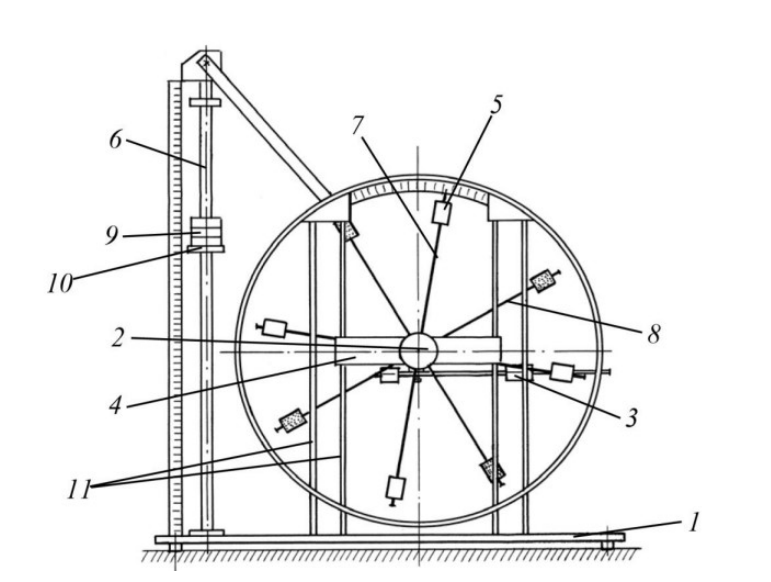
\includegraphics[width=10cm]{images/schema1}

    \smallvspace

    \textit{Рисунок 1.} Стенд лаборатории механики

\end{center}


В состав установки входят:

\begin{enumerate}
    \item Основание

    \item Рукоятка сцепления крестовин

    \item Устройства принудительного трения

    \item Поперечина

    \item Груз крестовины

    \item Трубчатая направляющая

    \item Передняя крестовина

    \item Задняя крестовина

    \item Шайбы каретки

    \item Каретка

    \item Система передних стоек
\end{enumerate}






    \clearpage

    \begin{center}
        \LARGE
        \textbf{Приложение 2. Таблицы измерений и расчётов}
    \end{center}

    \mediumvspace

    \begin{center}
    \begin{tabular}{|c|p{1.8cm}|p{1.8cm}|p{1.8cm}|p{1.8cm}|p{1.8cm}|p{1.8cm}|}
        \hline
        \multirow{2}{*}{Масса груза, г} & \multicolumn{6}{c|}{Положение утяжелителей} \\
        \cline{2-7}
        & 1 риска       & 2 риска & 3 риска & 4 риска & 5 риска & 6 риска \\
        \hline
        \multirow{4}{*}{$m_1$} & $t_1$         &         &         &         &         &         \\
        \cline{2-7}
        & $t_2$         &         &         &         &         &         \\
        \cline{2-7}
        & $t_3$         &         &         &         &         &         \\
        \cline{2-7}
        & $t_\text{ср}$ &         &         &         &         &         \\
        \hline
        \multirow{4}{*}{$m_2$} &               &         &         &         &         &         \\
        \cline{2-7}
        &               &         &         &         &         &         \\
        \cline{2-7}
        &               &         &         &         &         &         \\
        \cline{2-7}
        &               &         &         &         &         &         \\
        \hline
        \multirow{4}{*}{$m_3$} &               &         &         &         &         &         \\
        \cline{2-7}
        &               &         &         &         &         &         \\
        \cline{2-7}
        &               &         &         &         &         &         \\
        \cline{2-7}
        &               &         &         &         &         &         \\
        \hline
        \multirow{4}{*}{$m_4$} &               &         &         &         &         &         \\
        \cline{2-7}
        &               &         &         &         &         &         \\
        \cline{2-7}
        &               &         &         &         &         &         \\
        \cline{2-7}
        &               &         &         &         &         &         \\
        \hline

    \end{tabular}

    \smallvspace

    \textit{Таблица 2.} Протокол измерений времени падения груза при разной
    массе груза и разном положении утяжелителей на крестовине
\end{center}

    \begin{center}
    \hypertarget{table3}{}

    \renewcommand{\arraystretch}{1.8}

    \begin{tabular}{|c|C{2.5cm}|C{2.5cm}|C{1.8cm}|}
        \hline
         & \placeholder{$x - y$, м} & \placeholder{$2x - y$, м} & \placeholder{$\displaystyle \sqrt{\frac{a}{b}}$, с}  \\
        \hline
        1 & \placeholder{$0.540 \pm 0.065$}   & \placeholder{$0.840 \pm 0.500$}   & \placeholder{$7.5 \pm 1.1$}                       \\
        \hline
    \end{tabular}

    \smallvspace

    \textit{Таблица \placeholder{M}.} \placeholder{Какие-то интересные расчёты}

\end{center}

    \clearpage

    \begin{center}
        \LARGE
        \textbf{Приложение 3. Графики}
    \end{center}

    \mediumvspace

    \hypertarget{diagram1}{}

\begin{center}
    
\includegraphics[width=15cm]{images/logo}

    \smallvspace

    \textit{График 1.} \placeholder{Зависимость $ITMO = I(t) \cdot \frac{M}{O}$}
\end{center}



\end{document}